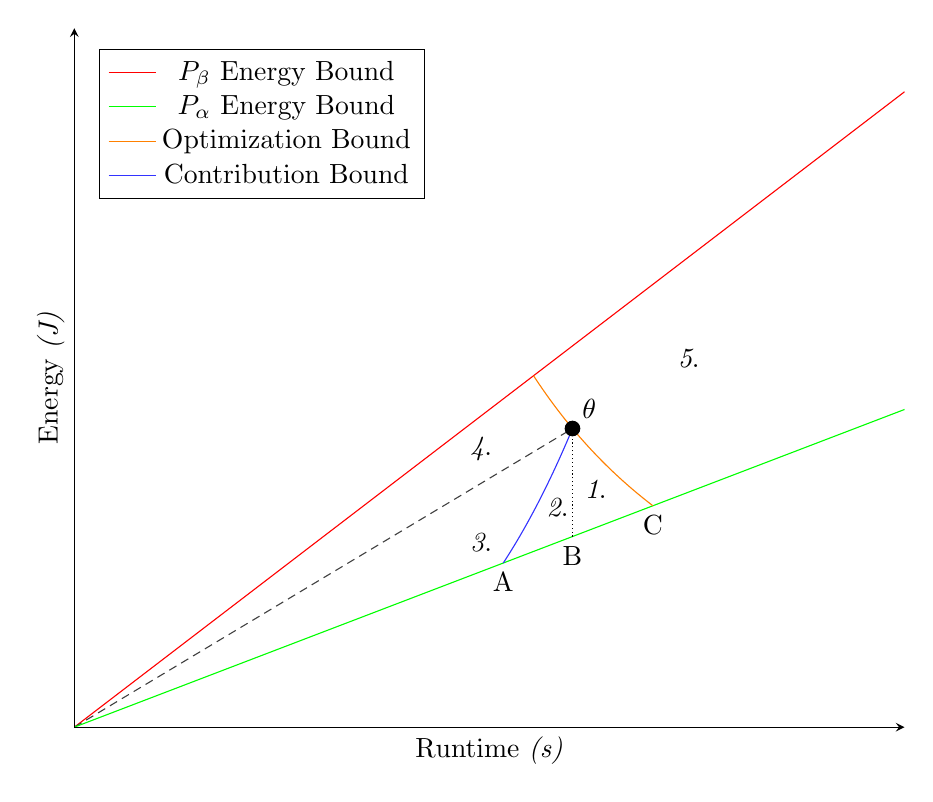
\begin{tikzpicture}
  \begin{axis}[ticks = none, 
    axis on top,
    axis x line=bottom,
    axis y line=left,
  	xlabel={Runtime \emph{(s)}},
    ylabel={Energy \emph{(J)}},    
    xmin=0, xmax=50,
    ymin=0, ymax=3300,
    width=\linewidth,
    legend style={legend pos=north west}
    ]

    %% Model Parameters %%
    \pgfmathsetmacro{\baselinepower}{30} % NOP code
    \pgfmathsetmacro{\rooflinepower}{60}
    \pgfmathsetmacro{\codepower}{47} 
    \pgfmathsetmacro{\codetime}{30}
    % Sadly, pgfplots sucks too much to calculate cube roots
    % These values are calculated with a ruby script in tools
    \pgfmathsetmacro{\anodex}{25.83028}
    \pgfmathsetmacro{\cnodex}{34.84283}
    \pgfmathsetmacro{\tnodex}{27.65477}

    \pgfmathsetmacro{\cnodey}{\cnodex * \baselinepower}
    \pgfmathsetmacro{\anodey}{\anodex * \baselinepower}
 
    %% Intermezzo Values %%
    \pgfmathsetmacro{\codeenergy}{\codepower * \codetime}
    \pgfmathsetmacro{\baselineenergy}{\baselinepower * \codetime}
    \pgfmathsetmacro{\rooflineenergy}{\rooflinepower * \codetime}
    \pgfmathsetmacro{\lowdisplayline}{(2 * \baselinepower + \codepower) / 3}
    \pgfmathsetmacro{\highdisplayline}{(1 * \rooflinepower + 1 * \codepower) / 2}

    % arguments: code power, code time, x - todo, apparently not supposed to do pgfmathparse
    \pgfmathdeclarefunction{metricbound}{3}{%
      \pgfmathparse{((#1 * #2^3) / #3^2)}%
    }
    \pgfmathdeclarefunction{definitionbound}{3}{%
      \pgfmathparse{((#1 / #2^3) * #3^4)}%
    }
     \pgfmathdeclarefunction{optimizationlimits}{3}{%
      \pgfmathparse{(min(metricbound(#1, #2, #3), definitionbound(#1, #2, #3)))}
    }

    % BETA ROOFLINE BOUND
    \addplot[color=red, domain=\pgfkeysvalueof{/pgfplots/xmin}:\pgfkeysvalueof{/pgfplots/xmax}] {\rooflinepower * x};
    \addlegendentry{$P_{\beta}$ Energy Bound}

    %const power diagonal
    \addplot[color=darkgray, densely dashed, forget plot, %forget plot prevents legend entry
            domain=\pgfkeysvalueof{/pgfplots/xmin}:\codetime] {\codepower * x}; 

    % ALPHA BASELINE BOUND 
    \addplot[color=green, domain=\pgfkeysvalueof{/pgfplots/xmin}:\pgfkeysvalueof{/pgfplots/xmax}] {\baselinepower * x};
    \addlegendentry{$P_{\alpha}$ Energy Bound} 

    \addplot[color=orange, domain=\tnodex:\cnodex] { metricbound(\codepower, \codetime, x)};
    \addlegendentry{Optimization Bound}

    \addplot[color=blue!80, domain=\anodex:\codetime] { definitionbound(\codepower, \codetime, x)};
    \addlegendentry{Contribution Bound}

    % Constant Time, Energy Dashes
    %vertical
    \draw[densely dotted] ({axis cs:\codetime,\baselineenergy}) -- ({axis cs:\codetime,\codeenergy});

    \node[circle,fill,inner sep=2pt] at (axis cs:\codetime,\codeenergy) {};
    \node[above right] at (axis cs:\codetime,\codeenergy) {$\theta$};
    \pgfmathsetmacro{\oneycoord}{\lowdisplayline * 31.4}
    \node at (axis cs:31.4,\oneycoord) {\textit1.};
    \pgfmathsetmacro{\twoycoord}{\lowdisplayline * 29.1}
    \node at (axis cs:29.1,\twoycoord) {\textit2.};
    \pgfmathsetmacro{\threeycoord}{\lowdisplayline * 24.5}
    \node at (axis cs:24.5,\threeycoord) {\textit3.};
    \pgfmathsetmacro{\fourycoord}{\highdisplayline * 24.5}
    \node at (axis cs:24.5,\fourycoord) {\textit4.};
    \pgfmathsetmacro{\fiveycoord}{\codepower * 37}
    \node at (axis cs:37,\fiveycoord) {\textit5.};
    
    \node [below] at ({axis cs:\anodex, \anodey}) {A};
    \node [below] at ({axis cs:\codetime,\baselineenergy}) {B};
    \node [below] at ({axis cs:\cnodex, \cnodey}) {C};
    %\node [below, name intersections={of=metric bound and baseline}] at (intersection-1) {C};


 \end{axis}
\end{tikzpicture}
